%%%%%%%%%%%%%%%
%
% $Autor: Gruppe 02 $
% $Datum: 2025-06 $
% $Projekt: Rundenzaehler fuer die Carrera-Bahn
% $Kurzbeschreibung: Beschreibung der einzelnen komponenten des Arduino Tiny Machine Learning Kits
% $Dateiname: ArduinoKit.tex
% $Abhängigkeiten: RundenzaehlerDoku.tex
%
%
%%%%%%%%%%%%%%%

\chapter{Arduino Tiny Machine Learning Kit}\label{ArduinoTinyMLKit}

Das Arduino Tiny Machine Learning Kit ist eine leistungsfähige Entwicklungsplattform, die es ermöglicht, Machine-Learning-Modelle direkt auf energieeffizienter Mikrocontroller-Hardware auszuführen. Im Mittelpunkt des Kits steht der Mikrocontroller Arduino Nano 33 BLE Sense Lite, der eine Vielzahl integrierter Sensoren für Beschleunigung, Temperatur, Luftdruck, Geräusche, Gesten und vieles mehr beinhaltet. \cite{ArduinoKit:2022}

Enthalten sind:

\begin{itemize}
	\item Arduino Nano 33 BLE Sense Lite
	\item Kameramodul (OV7675)
	\item Arduino Tiny Machine Learning Shield
	\item USB-A-auf-USB-Micro-Verbindungskabel
\end{itemize}

\begin{center}
	
\includegraphics[width=0.75\textwidth]{Nano33BLESense/TinyMLKit/TinyMachineLearningKit.png}
	\captionof{figure}{Arduino Tiny Machine Learning Kit\cite{ArduinoKit:2022}}
	\label{ArduinoKit}
\end{center}

\section{Arduino Nano 33 BLE Sense Lite}\label{chap:ArduinoNano33BLESenseLite}

Der Arduino Nano 33 BLE Sense Lite ist ein kompakt gebauter Mikrocontroller, der mit dem NINA B306 Funkmodul ausgestattet ist. Dieses Modul basiert auf dem Nordic nRF52840 Mikrocontroller und nutzt einen leistungsstarken Arm® Cortex-M4F® Prozessor. Zusätzlich verfügt es über einen integrierten Kryptografie-Chip, der eine sichere Speicherung von Zertifikaten und vorab geteilten Schlüsseln ermöglicht. Für Anwendungen im Bereich Bewegungserkennung bietet das Board außerdem eine 9-Achsen-Inertialsensorik (IMU). Die Platine kann flexibel entweder als steckbares Bauteil mit montierten Stiftleisten oder durch direktes Verlöten der wabenförmigen Kontaktflächen auf einer Leiterplatte verwendet werden.\cite{Arduino:2021}



Der Arduino Nano 33 BLE Sense Lite besitzt, wie alle Modelle der Nano-Serie, kein integriertes Ladesystem. Die Energieversorgung erfolgt wahlweise über die USB-Schnittstelle oder über die an den Stiftleisten verfügbaren Versorgungsanschlüsse.\cite{Arduino:2021}

Zu beachten ist, dass dieses Board ausschließlich mit 3,3\,V-Pegeln an seinen Ein- und Ausgängen arbeitet. Eine direkte Verbindung von 5-Volt-Signalen kann die Schaltung irreparabel beschädigen.\cite{Arduino:2021} 

Anders als bei älteren Arduino Nano-Versionen, bei denen der 5\,V-Pin eine stabile 5\,V-Versorgung bereitstellt, ist dieser Anschluss beim Nano 33 BLE Sense Lite nicht als Spannungsquelle nutzbar. Er ist lediglich intern mit dem USB-Eingang verbunden und führt nur dann Spannung, wenn das Board per USB mit Strom versorgt wird.\cite{Arduino:2021}

\subsection{Pinbelegung}
\label{PinbelegungTabelleArduino}
Die exakte Zuordnung der verfügbaren Pins des Arduino Nano 33 BLE Sense Lite wird in Abbildung~\ref{ArduinoPinbelegung} grafisch dargestellt. Eine detaillierte Übersicht über die Funktionen, Signaltypen und Anschlussmöglichkeiten der einzelnen Pins liefert Tabelle~\ref{tab:Pinbelegung}. Diese Informationen sind essenziell für die korrekte Anbindung externer Komponenten und die Planung von Schaltungen.
\begin{center}
	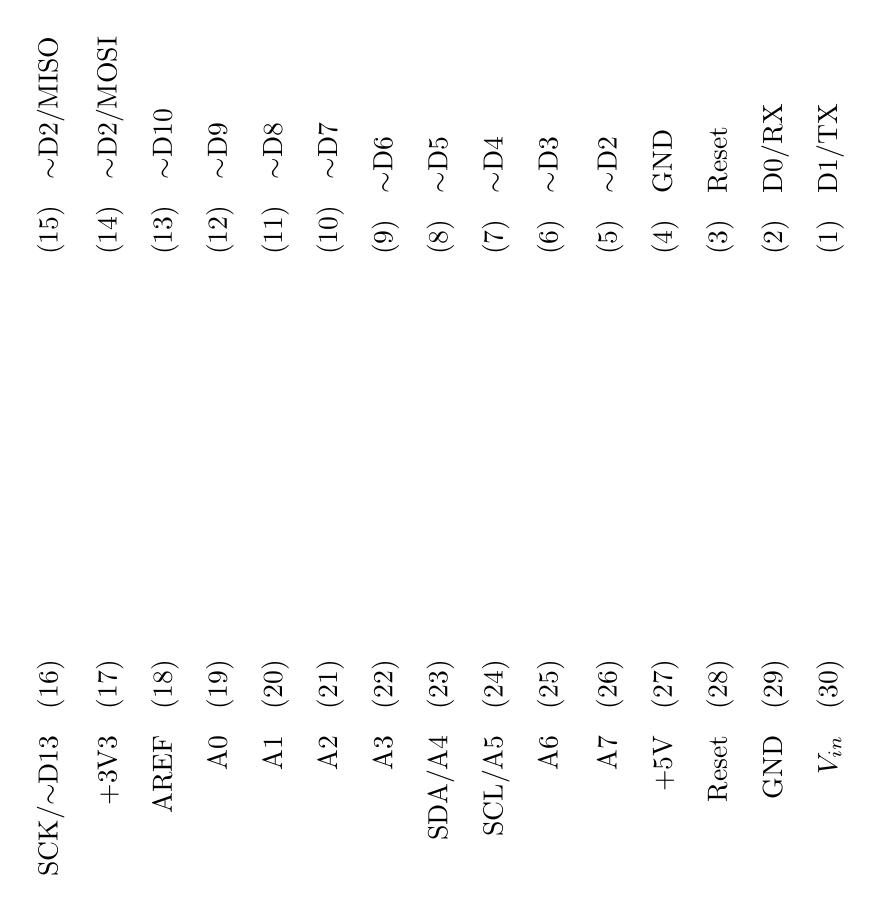
\begin{tikzpicture}
		
		\ArduinoNanoBLESenseRev
		
		\node[rotate=90,right] (Pin1) at (11.2,4.9) {(1) \; D1/TX};
		\node[rotate=90,right] (Pin2) at (10.5,4.9) {(2) \; D0/RX};
		\node[rotate=90,right] (Pin3) at (9.8,4.9) {(3) \; Reset};
		\node[rotate=90,right] (Pin4) at (9.1,4.9) {(4) \; GND};
		\node[rotate=90,right] (Pin5) at (8.4,4.9) {(5) \; $\sim$D2};
		\node[rotate=90,right] (Pin6) at (7.65,4.9) {(6) \; $\sim$D3};
		\node[rotate=90,right] (Pin7) at (6.95,4.9) {(7) \; $\sim$D4};
		\node[rotate=90,right] (Pin8) at (6.25,4.9) {(8) \; $\sim$D5};
		\node[rotate=90,right] (Pin9) at (5.55,4.9) {(9) \; $\sim$D6};
		\node[rotate=90,right] (Pin10) at (4.85,4.9) {(10) \; $\sim$D7};
		\node[rotate=90,right] (Pin11) at (4.15,4.9) {(11) \; $\sim$D8};
		\node[rotate=90,right] (Pin12) at (3.45,4.9) {(12) \; $\sim$D9};
		\node[rotate=90,right] (Pin13) at (2.75,4.9) {(13) \; $\sim$D10};
		\node[rotate=90,right] (Pin14) at (2.05,4.9) {(14) \; $\sim$D2/MOSI};
		\node[rotate=90,right] (Pin15) at (1.3,4.9) {(15) \; $\sim$D2/MISO};
		
		
		\node[rotate=90,left] (Pin30) at (11.2,-0.0) { $V_{in}$ \; (30)};
		\node[rotate=90,left] (Pin1) at (10.5,-0.0) {GND \; (29)};
		\node[rotate=90,left] (Pin2) at (9.8,-0.0) {Reset \; (28)};
		\node[rotate=90,left] (Pin3) at (9.1,-0.0) {+5V \; (27)};
		\node[rotate=90,left] (Pin4) at (8.4,-0.0) {A7 \; (26)};
		\node[rotate=90,left] (Pin5) at (7.65,-0.0) {A6 \; (25)};
		\node[rotate=90,left] (Pin6) at (6.95,-0.0) {SCL/A5 \; (24)};
		\node[rotate=90,left] (Pin7) at (6.25,-0.0) {SDA/A4 \; (23)};
		\node[rotate=90,left] (Pin8) at (5.55,-0.0) {A3 \; (22)};
		\node[rotate=90,left] (Pin9) at (4.85,-0.0) {A2 \; (21)};
		\node[rotate=90,left] (Pin10) at (4.15,-0.0) {A1 \; (20)};
		\node[rotate=90,left] (Pin11) at (3.45,-0.0) {A0 \; (19)};
		\node[rotate=90,left] (Pin12) at (2.75,-0.0) {AREF \; (18)};
		\node[rotate=90,left] (Pin13) at (2.05,-0.0) {+3V3 \; (17)};
		\node[rotate=90,left] (Pin14) at (1.3,-0.0) {SCK/$\sim$D13 \; (16)};
		
	\end{tikzpicture}
	\captionof{figure}{Arduino Pinbelegung}
	\label{ArduinoPinbelegung}
\end{center}

\begin{longtable}{|c|p{2cm}|c|p{6.5cm}|}
	\caption{Pinbelegung des Arduino Nano 33 BLE Sense\cite{Arduino:2021}}
	\label{tab:Pinbelegung} \\
	\hline
	\textbf{PIN} & \textbf{Funktion} & \textbf{Typ} & \textbf{Beschreibung} \\
	\hline
	\endfirsthead
	\hline
	\textbf{PIN} & \textbf{Funktion} & \textbf{Typ} & \textbf{Beschreibung} \\
	\hline
	\endhead
	\hline
	\endfoot
	
	\hline
	1 & D13 & Digital & GPIO\\
	\hline
	2 & +3V3 & Power Out & Intern erzeugte Stromausgabe an externe Geräte \\
	\hline
	3 & AREF & Analog & Analoge Referenz; kann als GPIO verwendet werden \\
	\hline
	4 & A0/DAC0 & Analog & ADC-Eingang/DAC-Ausgang, kann als GPIO verwendet werden\\
	\hline
	5 & A1 & Analog & ADC-Eingang; kann als GPIO verwendet werden \\
	\hline
	6 & A2 & Analog & ADC-Eingang; kann als GPIO verwendet werden\\
	\hline
	7 & A3 & Analog & ADC-Eingang; kann als GPIO verwendet werden \\
	\hline
	8 & A4/SDA & Analog & ADC-Eingang; I2C SDA; kann als GPIO verwendet werden \\
	\hline
	9 & A5/SCL & Analog & ADC-Eingang; I2C SCL; kann als GPIO verwendet werden \\
	\hline
	10 & A6 & Analog & ADC-Eingang; kann als GPIO verwendet werden \\
	\hline
	11 & A7 & Analog & ADC-Eingang; kann als GPIO verwendet werden \\
	\hline
	12 & VUSB & Power In/Out & Normalerweise NC; kann durch Kurzschließen eines Jumpers an den VUSB-Pin des USB-Anschlusses angeschlossen werden \\
	\hline
	13 & RST & Digital In & Aktiv-Low-Reset-Eingang (Duplikat von Pin 18)\\
	\hline
	14 & GND & Power & Strom Masse \\
	\hline
	15 & VIN & Power In & VIN Stromeingang \\
	\hline
	16 & TX & Digital & USART TX; Kann als GPIO verwendet werden \\
	\hline
	17 & RX & Digital & USART RX; Kann als GPIO verwendet werden \\
	\hline
	18 & RST & Digital & Aktiv-Low-Reset-Eingang (Duplikat von Pin 13) \\
	\hline
	19 & GND & Power & Strom Masse \\
	\hline
	20 & D2 & Digital & GPIO \\
	\hline
	21 & D3/PWM & Digital & GPIO; kann als PWM verwendet werden \\
	\hline
	22 & D4 & Digital & GPIO \\
	\hline
	23 & D5/PWM & Digital & GPIO; kann als PWM verwendet werden \\
	\hline
	24 & D6/PWM & Digital & GPIO; kann als PWM verwendet werden \\
	\hline
	25 & D7 & Digital & GPIO \\
	\hline
	26 & D8 & Digital & GPIO \\
	\hline
	27 & D9/PWM & Digital & GPIO; kann als PWM verwendet werden \\
	\hline
	28 & D10/PWM & Digital & GPIO; kann als PWM verwendet werden \\
	\hline
	29 & D11/MOSI & Digital & SPI MOSI; kann als GPIO verwendet werden \\
	\hline
	30 & D12/MISO & Digital & SPI MISO; kann als GPIO verwendet werden \\
	\hline
	
\end{longtable}

\subsection{Mechanik}
Formfaktor: Der Arduino Nano 33 BLE Sense hat einen kleinen Formfak
tor, der typischerweise etwa 45mm x 18mm misst, wobei Toleranzen von
etwa +/- 1mm möglich sind. Montagemöglichkeiten: Die Platine verfügt
über Bohrungen mit einem Durchmesser von etwa 3mm, wobei Toleranzen
von +/- 0,5mm möglich sind. \cite{Arduino:2021}

\subsection{Elektronik}
Prozessoreinheit: Der Arduino Nano 33 BLE Sense wird von einem 64 MHz
Arm Cortex-M4F Prozessor angetrieben, wobei die Taktfrequenz um bis
zu +/- 5 MHz variieren kann. NINA B306 Modul: Das integrierte NINA
B306 Modul bietet Bluetooth 5-Konnektivität mit einer Sendeleistung
von +8 dBm und Empfindlichkeit von-95 dBm, wobei Toleranzen von
+/- 1 dB möglich sind. \cite{Arduino:2021}

\subsection{Verbaute Sensoren}

\textbf{LSM9DS1 - Trägheitssensor:} Die Sensordaten haben eine Genauigkeit von etwa +/- 5 Prozent und eine Prozentual mögliche Messbereichs
toleranz von +/- 2 Prozent.
\\\\
\textbf{LPS22HB - Drucksensor:} Der Drucksensor hat eine Genauigkeit von etwa +/- 0,5 hPa und eine Temperaturgenauigkeit von etwa +/
0,2°C.
\\\\
\textbf{HTS221 - Feuchtigkeitssensor:} Die relative Feuchtigkeitsmessung hat eine Genauigkeit von etwa +/- 5 Prozent und eine Temperaturge
nauigkeit von etwa +/- 0,5°C.
\\\\
\textbf{APDS-9960 - Näherungs- und RGB-Sensor:} Die Näherungssensorgenauigkeit beträgt etwa +/- 2 mm, die RGB-Farberkennung hat eine Genauigkeit von etwa +/- 5 Prozent.
\\\\
\textbf{MP34DT05 - Digitales Mikrofon:} Die Genauigkeit des digitalen Mikrofons beträgt etwa +/- 2 dB.
\\\\
\textbf{ATECC608A - Kryptografischer Co-Prozessor:} Die kryptografische Funktion hat eine Genauigkeit von etwa +/- 1 Bit.
\\\\
\textbf{MPM3610 - DC-DC-Wandler:} Die Effizienz des DC-DC-Wandlers kann um bis zu +/- 5 Prozent variieren.
\\
\begin{center}
	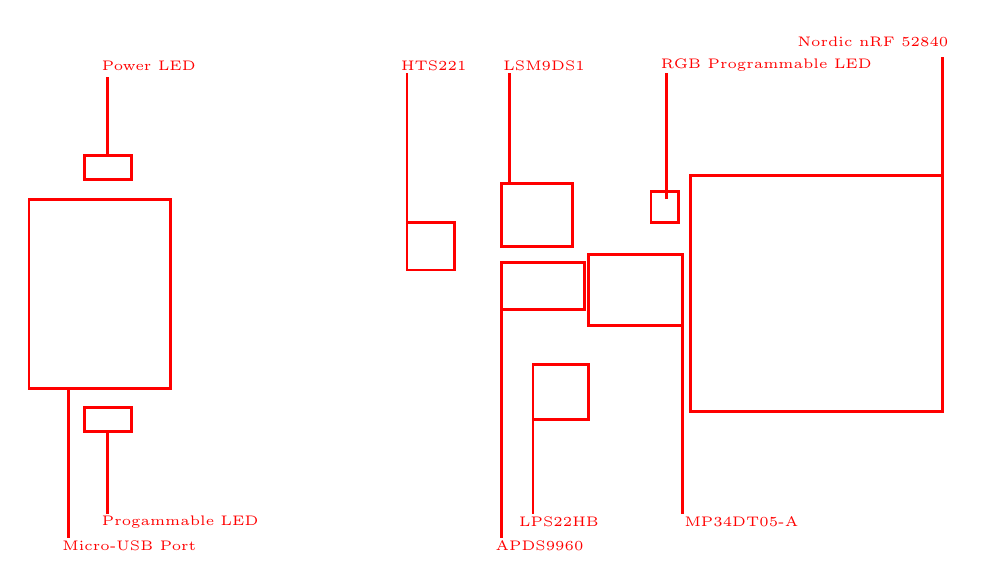
\begin{tikzpicture}
		\ArduinoNanoBLESenseOne
		
		\node[right](LEDPower) at (0.5,5.4){\textcolor{red}{\tiny Power LED}};
		\draw[line width=1pt,red]  (0.7,5.25) -- (0.7,4.25);
		\draw[line width=1pt,red] (0.4,4.25) -- (1.0, 4.25) -- (1.0,3.95) -- (0.4,3.95) -- cycle;
		
		\node[right](HTS) at (4.3,5.4){\textcolor{red}{\tiny HTS221}};
		\draw[line width=1pt,red]  (4.5,3.4) -- (4.5,5.3);
		\draw[line width=1pt,red] (4.5,3.4) -- (5.1, 3.4) -- (5.1,2.8) -- (4.5,2.8) -- cycle;
		
		\node[right](LSM9DS1) at (5.6,5.4){\textcolor{red}{\tiny LSM9DS1}};
		\draw[line width=1pt,red]  (5.8,3.9) -- (5.8,5.3);
		\draw[line width=1pt,red] (5.7,3.9) -- (6.6, 3.9) -- (6.6,3.1) -- (5.7,3.1) -- cycle;
		
		\node[right](RGB) at (7.6,5.4){\textcolor{red}{\tiny RGB Programmable LED}};
		\draw[line width=1pt,red]  (7.8,3.7) -- (7.8,5.3);
		\draw[line width=1pt,red] (7.6,3.8) -- (7.95, 3.8) -- (7.95,3.4) -- (7.6,3.4) -- cycle;
		
		\node[right](APD) at (5.5,-0.7){\textcolor{red}{\tiny APDS9960}};
		\draw[line width=1pt,red]  (5.7,2.3) -- (5.7,-0.6);
		\draw[line width=1pt,red] (5.7,2.9) -- (6.75, 2.9) -- (6.75,2.3) -- (5.7,2.3) -- cycle;
		
		\node[right](MP) at (7.9,-0.4){\textcolor{red}{\tiny MP34DT05-A}};
		\draw[line width=1pt,red]  (8,2.1) -- (8,-0.3);
		\draw[line width=1pt,red] (6.8,3.0) -- (8, 3.0) -- (8,2.1) -- (6.8,2.1) -- cycle;
		
		\node[left](HTS) at (11.5,5.7){\textcolor{red}{\tiny Nordic nRF 52840}};
		\draw[line width=1pt,red]  (11.3,4) -- (11.3,5.5);
		\draw[line width=1pt,red] (8.1,4) -- (11.3,4) -- (11.3,1) -- (8.1,1) -- cycle;
		
		\node[right](LPS) at (5.8,-0.4){\textcolor{red}{\tiny LPS22HB}};
		\draw[line width=1pt,red]  (6.1,1.0) -- (6.1,-0.3);
		\draw[line width=1pt,red] (6.1,0.9) -- (6.1,1.6) -- (6.8,1.6) -- (6.8,0.9) -- cycle;
		
		\node[right](LEDPower) at (0.5,-0.4){\textcolor{red}{\tiny Progammable LED}};
		\draw[line width=1pt,red]  (0.7,0.75) -- (0.7,-0.3);
		\draw[line width=1pt,red] (0.4,0.75) -- (1.0, 0.75) -- (1.0,1.05) -- (0.4,1.05) -- cycle;
		
		\node[right](USB) at (0,-0.7){\textcolor{red}{\tiny Micro-USB Port}};
		\draw[line width=1pt,red]  (0.2,1.3) -- (0.2,-0.6);
		\draw[line width=1pt,red] (-0.3,1.3) -- (-0.3, 3.7) -- (1.5,3.7) -- (1.5,1.3) -- cycle;
		
		
	\end{tikzpicture}
	\captionof{figure}{Arduino Nano 33 BLE Sense Architektur}\label{ArduinoNano33BLESenseArchitecture}
\end{center}
\newpage

\section{Tiny Machine Learning Shield}

Das Arduino Tiny Machine Learning Shield \ref{TinyMachineLearningShield1} ist eine Erweiterungsplatine, die speziell für den Arduino Nano 33 BLE Sense bzw. BLE Sense Lite entwickelt wurde. Das Shield besteht aus folgenden Komponenten: einer Grundplatine, zwei 15x1 Steckreihen für den Arduino, einer 10x2 Steckreihe für das Kamera Modul, sechs Grove-Anschlüssen, einer Anschlussklemme für eine externe Spannungsquelle und einen Taster. Sie ermöglicht eine standardisierte und robuste Verbindung mit verschiedenen Peripheriegeräten, insbesondere über das Grove-System. Dieses Stecksystem erlaubt eine einfache Integration von Sensoren und Aktoren ohne Lötarbeiten, was Entwicklungszeiten verkürzt und Fehler bei der Verdrahtung reduziert \cite{ArduinoKit:2022}.

\begin{center}
	
	\begin{tikzpicture}
		\ArduinoNanoShieldTikz
		
		
		\coordinate (A) at (6.61,28.14);
		\coordinate (B) at (7.45,24.81);    
		\begin{scope}
			\clip (A) rectangle (B);
			
			\ArduinoNanoShieldTikz
			
		\end{scope}
		
		
		%   \fill[black] (6.76, 27.97) rectangle (6.95, 27.76);
		\node[left] (Pin1) at (5.86,27.86) {\textcolor{white}{\tiny (1) \; +3V3}};
		\draw[line width=1pt,white] (6.86,27.86) -- (5.96,27.86);
		
		%   \fill[black] (7.09, 27.96) rectangle (7.29, 27.76);
		\node[right] (Pin1) at (8.2,27.86) {\textcolor{white}{\tiny (2) \; GND}};
		\draw[line width=1pt,white] (7.2,27.86) -- (8.1,27.86);
		
		%   \fill[black] (6.76, 27.64) rectangle (6.95, 27.44);
		\node[left] (Pin1) at (5.86,27.54) {\textcolor{white}{\tiny SCL \; (3)}};
		\draw[line width=1pt,white] (6.86,27.54) -- (5.96,27.54);
		
		%   \fill[black] (7.1, 27.63) rectangle (7.29, 27.44);
		\node[right] (Pin1) at (8.2,27.54) {\textcolor{white}{\tiny (4) \; SDA}};
		\draw[line width=1pt,white] (7.2,27.54) -- (8.1,27.54);
		
		%   \fill[black] (6.77, 27.33) rectangle (6.96, 27.13);
		\node[left] (Pin1) at (5.86,27.23) {\textcolor{white}{\tiny D8 \;  (5)}};
		\draw[line width=1pt,white] (6.86,27.23) -- (5.96,27.23);
		
		%   \fill[black] (7.1, 27.32) rectangle (7.29, 27.13);
		\node[right] (Pin1) at (8.2,27.23) {\textcolor{white}{\tiny (6) \; A1}};
		\draw[line width=1pt,white] (7.2,27.23) -- (8.1,27.23);
		
		%   \fill[black] (6.76, 27.02) rectangle (6.96, 26.82);
		\node[left] (Pin1) at (5.86,26.92) {\textcolor{white}{\tiny A0 \;  (7)}};
		\draw[line width=1pt,white] (6.86,26.92) -- (5.96,26.92);
		
		%   \fill[black] (7.1, 27.01) rectangle (7.29, 26.82);
		\node[right] (Pin1) at (8.2,26.92) {\textcolor{white}{\tiny (8)  \; D9}};
		\draw[line width=1pt,white] (7.2,26.92) -- (8.1,26.92);
		
		%   \fill[black] (6.77, 26.7) rectangle (6.96, 26.5);
		\node[left] (Pin1) at (5.86,26.6) {\textcolor{white}{\tiny D4 \; (9)}};
		\draw[line width=1pt,white] (6.86,26.6) -- (5.96,26.6);
		
		%   \fill[black] (7.1, 26.7) rectangle (7.29, 26.5);
		\node[right] (Pin1) at (8.2,26.6) {\textcolor{white}{\tiny (10) \; D6}};
		\draw[line width=1pt,white] (7.2,26.6) -- (8.1,26.6);
		
		%   \fill[black] (6.77, 26.39) rectangle (6.96, 26.19);
		\node[left] (Pin1) at (5.86,26.29) {\textcolor{white}{\tiny D5 \;  (11)}};
		\draw[line width=1pt,white] (6.86,26.29) -- (5.96,26.29);
		
		%   \fill[black] (7.11, 26.38) rectangle (7.3, 26.19);
		\node[right] (Pin1) at (8.2,26.29) {\textcolor{white}{\tiny (12) \; D3}};
		\draw[line width=1pt,white] (7.2,26.29) -- (8.1,26.29);
		
		%   \fill[black] (6.76, 26.08) rectangle (6.96, 25.87);
		\node[left] (Pin1) at (5.86,25.97) {\textcolor{white}{\tiny D2 \; (13)}};
		\draw[line width=1pt,white] (6.86,25.97) -- (5.96,25.97);
		
		%   \fill[black] (7.1, 26.07) rectangle (7.29, 25.87);
		\node[right] (Pin1) at (8.2,25.97) {\textcolor{white}{\tiny (14) \; D0}};
		\draw[line width=1pt,white] (7.2,25.97) -- (8.1,25.97);
		
		%   \fill[black] (6.76, 25.77) rectangle (6.95, 25.57);
		\node[left] (Pin1) at (5.86,25.67) {\textcolor{white}{\tiny D10 \;  (15)}};
		\draw[line width=1pt,white] (6.86,25.67) -- (5.96,25.67);
		
		%   \fill[black] (7.1, 25.76) rectangle (7.29, 25.57);
		\node[right] (Pin1) at (8.2,25.67) {\textcolor{white}{\tiny (16) \; D1}};
		\draw[line width=1pt,white] (7.2,25.67) -- (8.1,25.67);
		
		%   \fill[black] (6.76, 25.46) rectangle (6.95, 25.26);
		\node[left] (Pin1) at (5.86,25.36) {\textcolor{white}{\tiny (17)}};
		\draw[line width=1pt,white] (6.86,25.36) -- (5.96,25.36);
		
		%   \fill[black] (7.1, 25.45) rectangle (7.29, 25.26);
		\node[right] (Pin1) at (8.2,25.36) {\textcolor{white}{\tiny (18)}};
		\draw[line width=1pt,white] (7.2,25.36) -- (8.1,25.36);
		
		%   \fill[black] (6.76, 25.15) rectangle (6.96, 24.94);
		\node[left] (Pin1) at (5.86,25.05) {\textcolor{white}{\tiny Reset \; (19)}};
		\draw[line width=1pt,white] (6.86,25.05) -- (5.96,25.05);
		
		%   \fill[black] (7.1, 25.14) rectangle (7.29, 24.94);
		\node[right] (Pin1) at (8.2,25.05) {\textcolor{white}{\tiny (20) \; D11/MOSI}};
		\draw[line width=1pt,white] (7.2,25.05) -- (8.1,25.05);
		
		
	\end{tikzpicture}    
	
	%
\includegraphics[width=0.9\textwidth]{Nano33BLESense/TinyMLKit/TinyMachineLearningShieldRotated.png}
	\captionof{figure}{Das Tiny Machine Learning Shield \cite{ArduinoShield:2021}}\label{TinyMachineLearningShield1}
\end{center}

Die Pinbelegung für die Grove-Schnittstellen sind auf dem Tiny Machine Learning Shield beschriftet. Die Belegung für den 10-poligen Steckplatz für die Kamera ist in der Grafik \ref{TinyMachineLearningShieldPins1} dokumentiert. \\

\begin{center}
	
	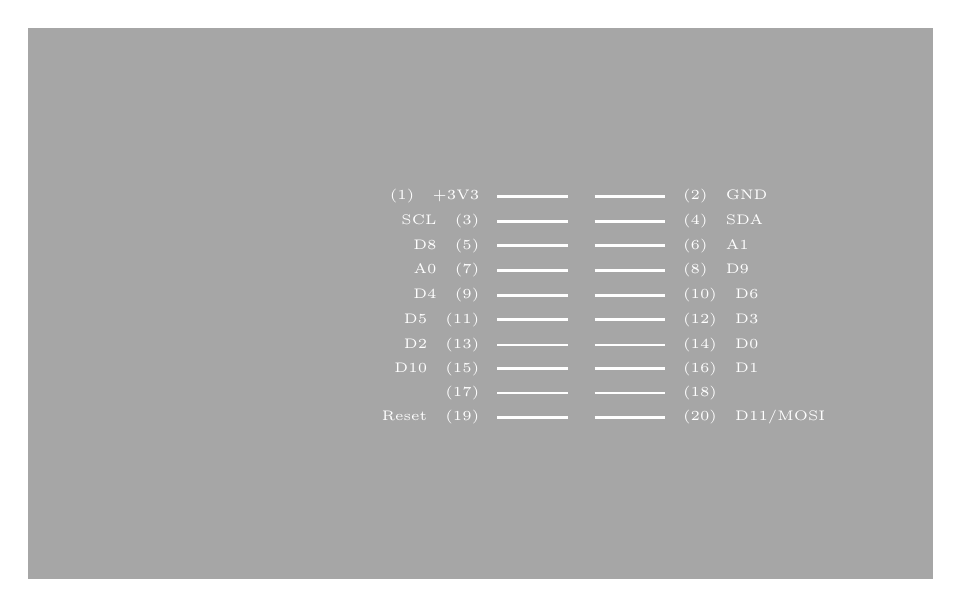
\begin{tikzpicture}
		\ArduinoNanoShieldTikz
		
		\fill[gray, opacity=0.7] (0,30) rectangle (11.5,23);
		
		
		\coordinate (A) at (6.61,28.14);
		\coordinate (B) at (7.45,24.81);    
		\begin{scope}
			\clip (A) rectangle (B);
			
			\ArduinoNanoShieldTikz
			
		\end{scope}
		
		
		%   \fill[black] (6.76, 27.97) rectangle (6.95, 27.76);
		\node[left] (Pin1) at (5.86,27.86) {\textcolor{white}{\tiny (1) \; +3V3}};
		\draw[line width=1pt,white] (6.86,27.86) -- (5.96,27.86);
		
		%   \fill[black] (7.09, 27.96) rectangle (7.29, 27.76);
		\node[right] (Pin1) at (8.2,27.86) {\textcolor{white}{\tiny (2) \; GND}};
		\draw[line width=1pt,white] (7.2,27.86) -- (8.1,27.86);
		
		%   \fill[black] (6.76, 27.64) rectangle (6.95, 27.44);
		\node[left] (Pin1) at (5.86,27.54) {\textcolor{white}{\tiny SCL \; (3)}};
		\draw[line width=1pt,white] (6.86,27.54) -- (5.96,27.54);
		
		%   \fill[black] (7.1, 27.63) rectangle (7.29, 27.44);
		\node[right] (Pin1) at (8.2,27.54) {\textcolor{white}{\tiny (4) \; SDA}};
		\draw[line width=1pt,white] (7.2,27.54) -- (8.1,27.54);
		
		%   \fill[black] (6.77, 27.33) rectangle (6.96, 27.13);
		\node[left] (Pin1) at (5.86,27.23) {\textcolor{white}{\tiny D8 \;  (5)}};
		\draw[line width=1pt,white] (6.86,27.23) -- (5.96,27.23);
		
		%   \fill[black] (7.1, 27.32) rectangle (7.29, 27.13);
		\node[right] (Pin1) at (8.2,27.23) {\textcolor{white}{\tiny (6) \; A1}};
		\draw[line width=1pt,white] (7.2,27.23) -- (8.1,27.23);
		
		%   \fill[black] (6.76, 27.02) rectangle (6.96, 26.82);
		\node[left] (Pin1) at (5.86,26.92) {\textcolor{white}{\tiny A0 \;  (7)}};
		\draw[line width=1pt,white] (6.86,26.92) -- (5.96,26.92);
		
		%   \fill[black] (7.1, 27.01) rectangle (7.29, 26.82);
		\node[right] (Pin1) at (8.2,26.92) {\textcolor{white}{\tiny (8)  \; D9}};
		\draw[line width=1pt,white] (7.2,26.92) -- (8.1,26.92);
		
		%   \fill[black] (6.77, 26.7) rectangle (6.96, 26.5);
		\node[left] (Pin1) at (5.86,26.6) {\textcolor{white}{\tiny D4 \; (9)}};
		\draw[line width=1pt,white] (6.86,26.6) -- (5.96,26.6);
		
		%   \fill[black] (7.1, 26.7) rectangle (7.29, 26.5);
		\node[right] (Pin1) at (8.2,26.6) {\textcolor{white}{\tiny (10) \; D6}};
		\draw[line width=1pt,white] (7.2,26.6) -- (8.1,26.6);
		
		%   \fill[black] (6.77, 26.39) rectangle (6.96, 26.19);
		\node[left] (Pin1) at (5.86,26.29) {\textcolor{white}{\tiny D5 \;  (11)}};
		\draw[line width=1pt,white] (6.86,26.29) -- (5.96,26.29);
		
		%   \fill[black] (7.11, 26.38) rectangle (7.3, 26.19);
		\node[right] (Pin1) at (8.2,26.29) {\textcolor{white}{\tiny (12) \; D3}};
		\draw[line width=1pt,white] (7.2,26.29) -- (8.1,26.29);
		
		%   \fill[black] (6.76, 26.08) rectangle (6.96, 25.87);
		\node[left] (Pin1) at (5.86,25.97) {\textcolor{white}{\tiny D2 \; (13)}};
		\draw[line width=1pt,white] (6.86,25.97) -- (5.96,25.97);
		
		%   \fill[black] (7.1, 26.07) rectangle (7.29, 25.87);
		\node[right] (Pin1) at (8.2,25.97) {\textcolor{white}{\tiny (14) \; D0}};
		\draw[line width=1pt,white] (7.2,25.97) -- (8.1,25.97);
		
		%   \fill[black] (6.76, 25.77) rectangle (6.95, 25.57);
		\node[left] (Pin1) at (5.86,25.67) {\textcolor{white}{\tiny D10 \;  (15)}};
		\draw[line width=1pt,white] (6.86,25.67) -- (5.96,25.67);
		
		%   \fill[black] (7.1, 25.76) rectangle (7.29, 25.57);
		\node[right] (Pin1) at (8.2,25.67) {\textcolor{white}{\tiny (16) \; D1}};
		\draw[line width=1pt,white] (7.2,25.67) -- (8.1,25.67);
		
		%   \fill[black] (6.76, 25.46) rectangle (6.95, 25.26);
		\node[left] (Pin1) at (5.86,25.36) {\textcolor{white}{\tiny (17)}};
		\draw[line width=1pt,white] (6.86,25.36) -- (5.96,25.36);
		
		%   \fill[black] (7.1, 25.45) rectangle (7.29, 25.26);
		\node[right] (Pin1) at (8.2,25.36) {\textcolor{white}{\tiny (18)}};
		\draw[line width=1pt,white] (7.2,25.36) -- (8.1,25.36);
		
		%   \fill[black] (6.76, 25.15) rectangle (6.96, 24.94);
		\node[left] (Pin1) at (5.86,25.05) {\textcolor{white}{\tiny Reset \; (19)}};
		\draw[line width=1pt,white] (6.86,25.05) -- (5.96,25.05);
		
		%   \fill[black] (7.1, 25.14) rectangle (7.29, 24.94);
		\node[right] (Pin1) at (8.2,25.05) {\textcolor{white}{\tiny (20) \; D11/MOSI}};
		\draw[line width=1pt,white] (7.2,25.05) -- (8.1,25.05);
		
		
	\end{tikzpicture}  
	\captionof{figure}[Pin-Belegung des Tiny Machine Learning Shields]{Pin-Belegung des Tiny Machine Learning Shields \cite{ArduinoShield:2021}}\label{TinyMachineLearningShieldPins1}
\end{center}

\Ausblenden{
	\begin{center}
		
\includegraphics[width=0.75\textwidth]{Nano33BLESense/TinyMLKit/TinyMachineLearningShield.png}
		\captionof{figure}{Arduino Tiny Machine Learning Shield\cite{ArduinoKit:2022}}
		\label{TinyMachineLearningShield}
	\end{center}
}
\newpage

\subsection{Mechanische Eigenschaften}

\begin{itemize}
	\item \textbf{Maße:} ca. 45 mm × 32 mm \cite{ArduinoKit:2022}
	
	\item \textbf{Bohrlöcher:} 3 mm Durchmesser zur Fixierung in Gehäusen oder auf Trägerplatten \cite{ArduinoKit:2022}
	
	\item \textbf{Montage:} der Arduino Nano wird direkt über Pins aufgesteckt \cite{ArduinoKit:2022}
\end{itemize}

\subsection{Spannungsversorgung}
\label{Spannungsversorgung}

Das Shield bietet einen JST-PH-Anschluss zur Verbindung externer Stromquellen. Der integrierte Schalter ermöglicht das gezielte Ein- und Ausschalten der Stromversorgung, ohne den USB-Stecker zu entfernen \cite{ArduinoKit:2022}.
\textbf{Folgende Versorgungsvarianten sind möglich:}

\begin{itemize}
	
	\item USB-Stromversorgung über den Arduino Nano
	
	\item Externe Versorgung über JST-PH-Buchse 
	
\end{itemize}

\textbf{Achtung:} Es ist kein interner Verpolungsschutz verbaut. Es ist also genau darauf zu achten, dass die Pole bei einer externen Spannungsversorgung korrekt angeschlossen sind \cite{ArduinoKit:2022}.

\begin{center}
	
\includegraphics[width=0.35\textwidth]{Grove/Grove2Pin}
	\captionof{figure}{Grove 4-Pin Kabel \cite{Reichelt:2024g}}
	\label{JST_Kabel}
\end{center}

\section{Kameramodul ArduCam OV7675}

Das im Tiny Machine Learning Kit beigelegte Kamera Modul \ref{Kameramodul} der Firma ArduCam ergänzt die Bilderfassungsfähigkeiten des Arduino. Dieser besitzt zwar fest verbaute Licht-, Helligkeit- und Farbsensoren, allerdings keine eigene Videoerfassung. Dies kann durch das Kamera Modul ArduCam OV7675 realisiert werden \cite{ArduCam:2024}, welches auf die dafür vorgesehenen Anschlüsse auf dem custom Arduino Tiny Machine Learning Shield gesteckt werden kann. Für den Rundenzähler wird das Kameramodul nicht verwendet. Aus diesem Grund wird auf eine ausführliche Beschreibung und Dokumentation verzichtet. 

\begin{center}
	
\includegraphics[width=0.65\textwidth]{Nano33BLESense/TinyMLKit/OV7675}
	\captionof{figure}{Kamera ArduCam 0V7675 \cite{ArduCam:2024}}
	\label{Kameramodul}
\end{center}


\subsection{Kabel USB-A auf USB-B}
Das USB-A auf USB-Micro-B Kabel \ref{USB_Kabel} ist eine Verbindungslösung, die es ermöglicht, Geräte mit einem USB-Anschluss Typ A mit Geräten mit einem USB-Micro-B-Anschluss zu verbinden. Das Kabel ist vielseitig einsetzbar und eignet sich ideal für den Anschluss von Smartphones, Tablets, Kameras, externen Festplatten und anderen elektronischen Geräten an Computer, Laptops, Ladegeräte und andere USB-Host-Geräte.
Es ermöglicht die Übertragung von Daten, das Laden von Geräten und den Zugriff auf verschiedene Funktionen und Anwendungen.
\begin{center}
	
\includegraphics[width=0.65\textwidth]{Nano33BLESense/TinyMLKit/USBCable}
	\captionof{figure}{USB-A auf USB-Micro-B Kabel \cite{Arduino:2021}}
	\label{USB_Kabel}
\end{center}
\newpage